\documentclass[runningheads,a4paper]{llncs}
\usepackage[utf8]{inputenc}
\usepackage[english]{babel}
\usepackage{pdfpages, titling}
\usepackage{array, float}
\usepackage{multicol, booktabs}
\usepackage{cite, tablefootnote}
\usepackage{graphicx, caption, subfigure, wrapfig}
\usepackage{listings}
\usepackage{geometry}
\usepackage{color}
\usepackage{mathtools, braket}
\usepackage{amssymb}
\usepackage[nottoc]{tocbibind} % references in the toc
\usepackage{etoolbox}

\geometry{
	includeheadfoot,
    margin=2.54cm
}

\usepackage{footnote}
\makesavenoteenv{tabular}
\makesavenoteenv{table}

\usepackage{textcomp}
\usepackage{minted}
\usepackage[hidelinks]{hyperref}
\graphicspath{{Pictures/}} % Specifies the directory where pictures are stored/

\newcommand{\vect}[1]{\boldsymbol{#1}}
\renewcommand{\subtitle}[1]{
  \posttitle{
    \par\end{center}
    \begin{center}\large#1\end{center}
    \vskip0.5em}
}

\author{Jaro Camphuijsen (jcn690), Rahiel Kasim (rkm700), Jan Westerdiep (jwp800)}
\date{\today}
\title{Process Report}
\subtitle{Databeestjes - Group 091}
\patchcmd{\thebibliography}{\chapter*}{\section*}{}{}
\begin{document}
\maketitle

\section{Schedule and Contribution}
Starting with some exploration on the 4th of May and another day of exploration on the 11th of May, the real work was done in a period between the 23rd and 29th of May. In this last period, every day the model improved and the report grew. In Table~\ref{table:schedule} you can find the tasks and contributions per day. 

\begin{table}
\centering
    \begin{tabular}{ l||l|l|l }    
    \toprule
    \textbf{Date}                	& \textbf{Jan}                & \textbf{Rahiel}   			& \textbf{Jaro}                      \\ \midrule
May 4 & N/A & \multicolumn{2}{c}{Start up project, business understanding, data exploration} \\
May 11& Data exploration and report & data exploration and report & N/A \\
May 23& Getting RankPy to work & N/A & N/A\\
May 24& Exploration & writing intro & exploration \\
May 25& Feature engineering, RankLib, RankPy & related work & feature exploration and design \\
May 26& Report: models & report: features & report: features \\
May 27& RankLib, training, report & feature engineering & N/A \\
May 28& Report, training & N/A & N/A\\
May 29& Report, training, compare models & report & report, process report \\ \bottomrule
    \end{tabular}
    \caption{A summary of the work done per team member per working day.}
	\label{table:schedule}
\end{table}

As we used git to share and work on code with multiple members \footnote{Databeestjes. \url{https://github.com/sunsistemo/databeestjes}}, we can use the GitHub web interface to get some statistics about the code contributions. It should be noted however that this does not explicitly mean that the major contributor on GitHub did the majority of the work on the whole project.

In Figure~\ref{fig:gh_contrib}, the time line of GitHub commits is shown. We clearly see the major contribution of Jan as he was appointed the task to implement the actual algorithm, while Rahiel and Jaro would focus on the report and research. We would however meet up often and discuss the options with all members at the meeting before implementing it. 

As a start we tried to get the python benchmark from Kaggle to work on our data set. It uses a random tree algorithm. 
Early on we decided to put our effort into getting a LambdaMART implementation to work and we started out using the RankPy library which has a LambdaMART implementation in it. When this was working we decided we wanted to test it against some other methods. This was when we started on trying RankLib which incorporates several other ranking algorithms which you can access with similar interfaces. 

\begin{figure}[h]
	\centering
	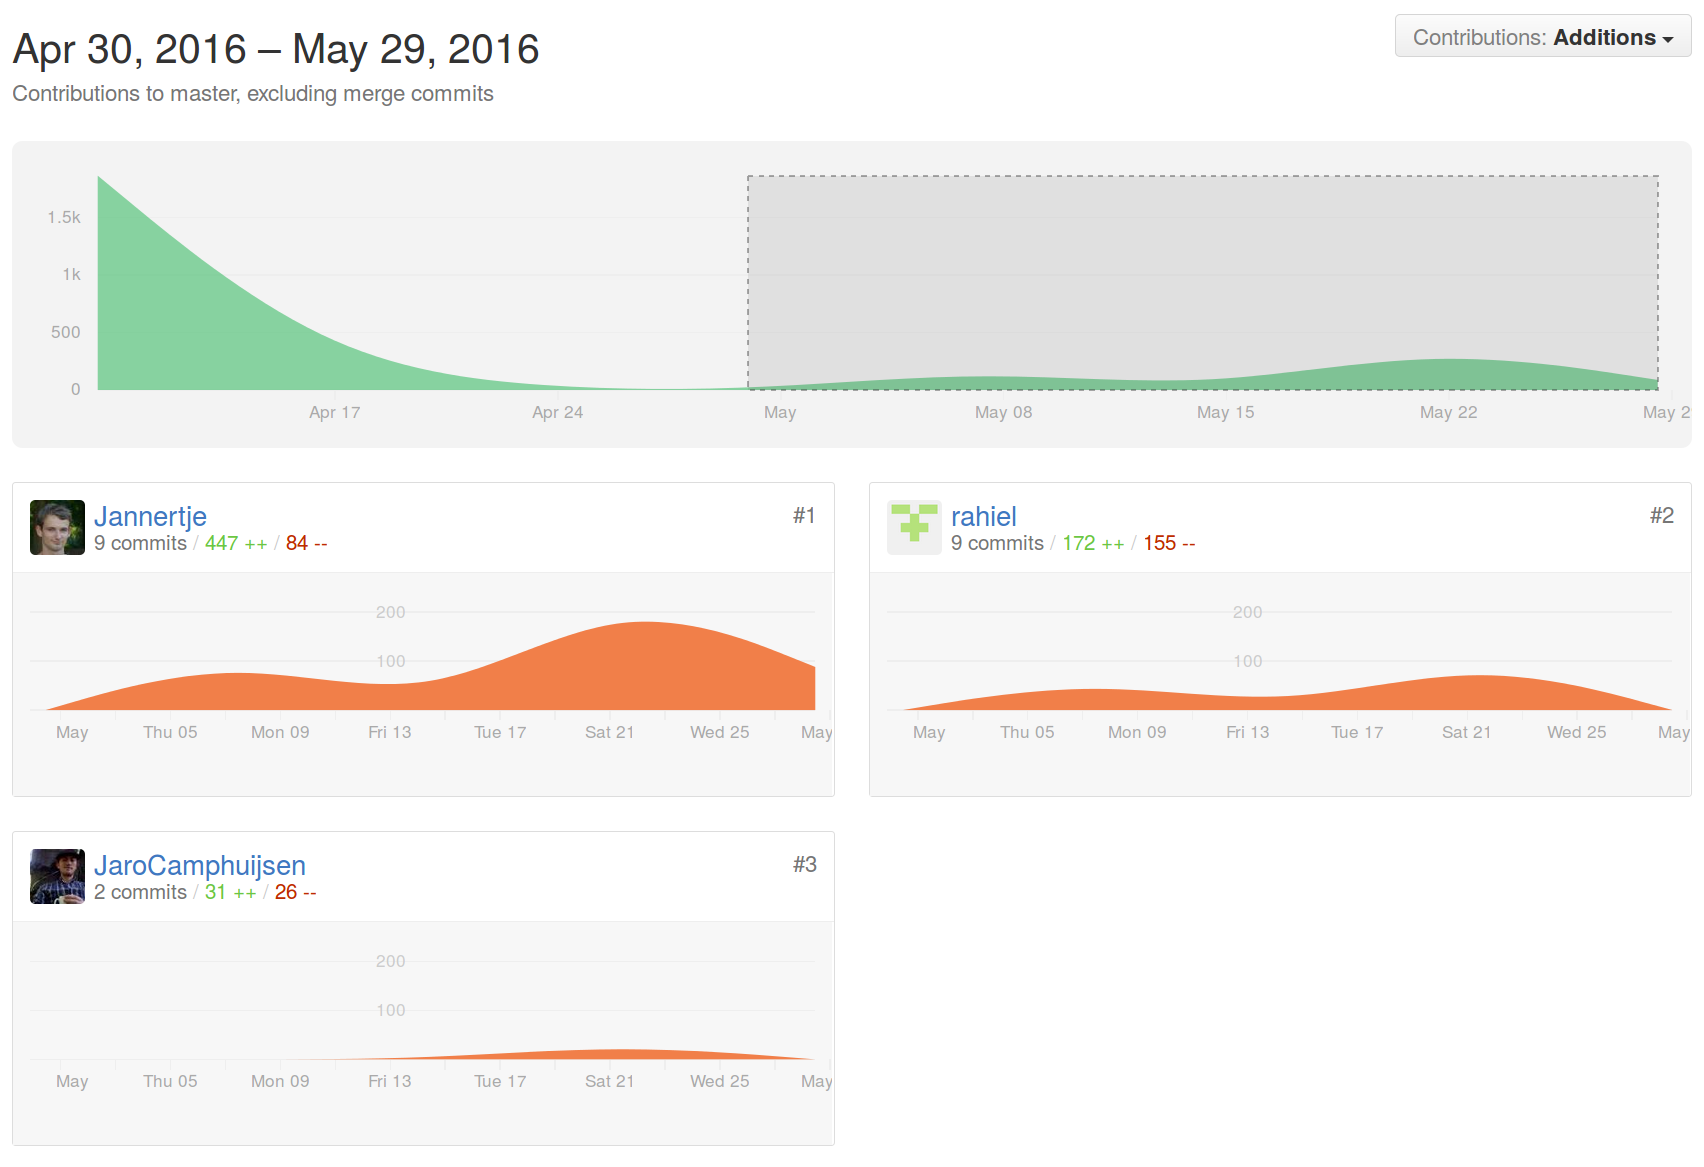
\includegraphics[width=14cm]{Pictures/contributions2.png}
    \caption{Contribution to the model on GitHub in total (top) and per team member.}
    \label{fig:gh_contrib}
\end{figure}

\section{Discussion}
The first thing to note from the schedule in table \ref{table:schedule} is the timing of our first meeting which is only on the 4th of May while we received the assignment already in April. Even after this first meeting nothing happens for a while until the 23rd of May (six days before the deadline) from which day on we work on it every day. One could question if this is the most desired approach of working on a project. 

If we look at the attendance in the schedule. Jan and Rahiel were at most of the meetings and 
Jaro missed four of them. Due to an external commitment he could attend less of the meetings and was forced to concentrate less on this assignment than his fellow team members. Besides this unfortunate double booking, the cooperation was good: we mostly worked physically together so we could benefit from each others knowledge when we got stuck. This also made discussing issues easy. 

Using git we could easily edit the same script and with the use of overleaf (an online interactive \LaTeX editor) it was possible to simultaneously work on the same \LaTeX-file. At some of the earlier meetings we would also start with an overview of the assignment and how we should divide tasks. This became less needed as the project evolved and team members could easily pickup where others left off.  

\section{Future work}
Because Figure~\ref{fig:gh_contrib} in this specific case actually reflects our contribution ranking, Rahiel and Jaro decided to share the load and relieve Jan from the presentation task since he was clearly the number one contributor of this project. They will prepare and give the presentation together instead of all three. 

\end{document}

4 May: jaro + rahiel read assignment, find presentations of the kaggle competition winners, start on business understanding and data exploration
11 may: jan + rahiel: data exploration and writing
23 may: jan: getting LambdaMART to work
24 may: jan + jaro: exploration, rahiel: intro
25 may: jan: feature engineering, ranklib, rahiel: related work, jaro: feature exploration/design
26 may: jan: report, models; rahiel: report, features; jaro: report
27 may: jan: ranklib, training, report; rahiel: features
28 may: jan: report, training
29 may: jan: report, training; Rahiel: ; Jaro: report, writing proces report



